\documentclass[a4paper, 12pt]{book}
\usepackage{graphicx}
\usepackage[french]{babel}
\usepackage[utf8]{inputenc}
\usepackage{textcomp}
\usepackage[T1]{fontenc}
\usepackage{multirow}

\usepackage[table]{xcolor}

\usepackage{listings}
\usepackage{float}
\usepackage{url}
\usepackage[french]{algorithm}
\usepackage{style/myalgorithm}
\usepackage{amsmath,amsfonts,amssymb}
\usepackage{biblatex}
\addbibresource{memoire}
\newcommand{\fBm}{\emph{fBm}~}
\newcommand{\etal}{\emph{et al.}~}
\newcommand{\glAd}{\emph{GL4D}~}
\newcommand{\apiopengl}{API OpenGL\textsuperscript{\textregistered}~}
\newcommand{\opengl}{OpenGL\textsuperscript{\textregistered}~}
\newcommand{\opengles}{OpenGL\textsuperscript{\textregistered}ES~}
\newcommand{\clang}{langage \texttt{C}}
\newcommand{\codesource}{\textsc{Code source}~}
\floatstyle{ruled}
\newfloat{programslist}{htbp}{locs}
\newcommand{\listofprograms}{\listof{programslist}{Liste des codes source}}
\newcounter{program}[subsection]
\renewcommand{\theprogram}{\arabic{chapter}.\arabic{program}}

\newenvironment{program}[1]{
  \if\relax\detokenize{#1}\relax
  \gdef\mycaption{\relax}
  \else
  \gdef\mycaption{#1}
  \fi
  \refstepcounter{program}
  \addcontentsline{locs}{section}{#1}
  \footnotesize
}{
  \begin{description}
    \item[\codesource \theprogram]--~\mycaption
  \end{description}
}

\begin{document}
\begin{titlepage}
  \begin{center}
    %\begin{tabular*}{\textwidth}{l@{\extracolsep{\fill}}r}
      
\includegraphics[height=2.5cm, width=6cm]{images/paris8Logo.png}
    %\end{tabular*}
    \small 
    \rule{\textwidth}{.5pt}~\\
    \large 
    \textsc{Université Paris 8 - Vincennes à Saint-Denis}\vspace{0.5cm}\\
    \textbf{Licence Informatique}\vspace{3.0cm}\\
    \Large
    \textbf{Mémoire de projet tuteuré}\\
    \textbf{Qualification de caméras RGB-D}\vspace{1.5cm}\\
    
    \large
    \textbf{Yasmine BOUDJEMAÏ}\\
    \textbf{Mélanie DE JESUS CORREIA}\vspace{1.5cm}\\
  \end{center}\vspace{3.5cm}~\\
  \begin{tabular}{ll}
    \hspace{-0.45cm}Organisme d'accueil~:~&~Université Paris 8 Vincennes-Saint-Denis\\
    \hspace{-0.45cm}Tuteur -- Organisme d'accueil~:~&~Farès  \textsc{BELHADJ}\\
  \end{tabular}
\end{titlepage}
\frontmatter



\chapter*{Dédicaces}
\markboth{\sc Dédicaces}{}
\addcontentsline{toc}{chapter}{Dédicaces}
À la mémoire de mon très cher frère bien-aimé \emph{\textbf{Belkacem}} qui a contribué pleinement à ma réussite sur différents plans. Pour son grand soutien moral et intellectuel que je n'oublierai jamais . Pour tous les moments de complicité passés dans des ambiances où bonheur, joie et rire s'entremêlaient. Il était tel un troisième parent pour moi, se souciant constamment de mon bien-être. Il était également tel un frère jumeau car ressentant quand j'avais besoin de soutien et d'aide ne serait-ce que minime était-elle. Ainsi que pour toutes les autres choses qu'il a su m'apporter que la page ne pourrait citer.


\chapter*{Remerciements}
\markboth{\sc Remerciements}{}
\addcontentsline{toc}{chapter}{Remerciements} Je tiens à remercier toutes les personnes qui m'ont apporté une quelconque contribution durant ce stage.\\
\par Je souhaiterais tout d'abord adresser mes sincères remerciements à mon maître de stage \textbf{M.Farès BELHADJ} pour m'avoir accordée sa confiance pour les missions sollicitées. Ainsi que de m'avoir aidée lors de la conception du modèle réel et virtuel et pour tous ses conseils précieux qui ont été utiles pour le bon déroulement du stage. \\
\par Par ailleurs, je voudrais remercier \textbf{Mme.Martine LE LEZ} pour m'avoir aidée pour la recherche de stage.\\
\par Enfin, je voudrais exprimer toute ma reconnaissance et toute ma gratitude envers toute ma famille. Un grand merci pour mes parents pour leur soutien moral quotidien inestimable. Je souhaite également remercier mes frères ainsi que ma belle-sœur et mon petit neveu pour leurs contributions lors de la réalisation du modèle réel. 

\chapter*{Résumé}
\markboth{\sc Résumé}{}
\addcontentsline{toc}{chapter}{Résumé} 
Dès lors de sa sortie, de nombreux domaines ont connu un essor important à l 'aide des technologies RGB-D. À titre d'exemple, on peut citer NaturalPad \footnote{Entreprise, basée à Montpellier, spécialisée dans la création de jeux vidéo ludiques au service des besoins médicaux.} qui se sert de la Kinect pour la capture de mouvements pour des besoins de rééducation.	
\par Dans des applications où la précision demeure nécessaire pour de meilleurs résultats, il est indispensable de savoir choisir le capteur qui convient le mieux aux exigences du contexte de l'application.
Dans ce document, nous expliquons comment nous avons réalisé notre application pour qualifier un ensemble de caméras RGB-D. Nous exposons les résultats produits par notre application, puis discutons de de la fiabilité des résultats obtenus.
\par Dans le premier chapitre, nous proposons un état de l'art des technologies de la caméra RGB-D. Dans le second, nous détaillons les étapes par lesquelles nous sommes passés pour élaborer l'outil répondant à la demande du stage, ainsi que les résultats obtenus. Dans le troisième, nous montrons comment procéder pour utiliser un modèle bien précis de caméra afin de démarrer les tests avec ce dernier. Enfin, en conclusion, nous exposons succinctement le bilan du travail réalisé.


%% Table des matières
\tableofcontents
%% La liste des figure est optionnelle (si votre rapport manque de
%% contenu ajouter ce type de pages sera perçu négativement)
\listoffigures
%% La liste des programmes est optionnelle (si votre rapport manque de
%% contenu ajouter ce type de pages sera perçu négativement)
%\listofprogram
\mainmatter
\chapter*{Introduction}
\markboth{\sc Introduction}{}
\addcontentsline{toc}{chapter}{Introduction}
La caméra RGB-D dans ses débuts, notamment la Kinect, a beaucoup servi le monde du jeux-vidéo. Cependant, depuis un certain nombre d'années, elle contribue activement et fondamentalement dans le développement de multiples applications dans diverses disciplines telles que la médecine, la robotique et plus généralement l'aide à la personne.
\par Ce stage, effectué au sein de l'Université Paris 8 Vincennes-Saint-Denis, a pour objet la conception d'outils pour la qualification de caméras RGB-D. Il vise à comparer différentes caméras afin de sélectionner la meilleure en fonction du besoin ciblé.
\par Tout d'abord, avant de passer à l'étape des qualifications,  il nous faut concevoir un modèle-étalon sur lequel nous passerons nos tests de mesure. Ce dernier est fait principalement de polystyrène. Ensuite,   nous fabriquons sa version virtuelle en 3D en ayant recours au logiciel \emph{123D Design}.
\par Par la suite, nous exploitons certaines fonctions OpenCV telles que matchTemplate afin de détecter le modèle-étalon.
\par Enfin, nous opposons les données OpenGL et les données des caméras que nous avons pu réunir à partir de l'aire du modèle détecté en se servant de méthodes différentes pour le calcul du taux d'erreurs tel que le RMSE (Root Mean Square Error) \footnote{Méthode permettant de calculer l'écart-type des erreurs enregistrées. Se reférer à cette page web pour davantage de renseignements: \url{https://www.statisticshowto.datasciencecentral.com/rmse/}}. L'application produit automatiquement un rapport mettant en avant ces divergences.
\chapter{État de l'art}

Dans ce chapitre, nous allons définir ce qu'est une caméra RGB-D, nous énumérons certains des différents modèles existants que nous comptons utiliser pour ce projet, nous abordons brièvement les différentes techniques utilisées pour la récupération de la profondeur par une caméra. Enfin, nous discutons les différences recensées sur la \texttt{kinect V2} et \texttt{V3}.

\section{Description d'une caméra RGB-D}

La caméra RGB-D, aussi appelée capteur RGB-D, comprend un capteur RGB et un capteur de profondeur (D pour Depth). Ces derniers capturent des images couleur ainsi que des informations de profondeur par pixel. C'est principalement ces dernières qui vont nous intéresser tout au long des qualifications.


\section{Modèles existants}
Il existe différents modèles de caméras RGB-D. Parmi elles, nous pouvons citer la Kinect et ses différentes versions, Asus Xtion Pro Live, BlasterX Senz3D, Orbbec, Intel RealSense D415, ... 
\par \texttt{Kinect} a fait son apparition en septembre 2008. Elle a été conçue par Microsoft et était destinée pour les consoles de jeux XBox 360. Elle permettait aux utilisateurs d'interagir avec la console à l'aide d'une NUI \footnote{Natural User Interface (Interface Utilisateur Naturelle), se réfère à une interface utilisateur invisible.} en utilisant les mouvements gestuels et une reconnaissance vocale. Elle sera plus tard utilisée dans les domaines de la  recherche et du développement pour différents secteurs comme le domaine de la médecine, l'industrie automobile, la robotique, l'éducation,  .... 
\par \texttt{Asus Xtion Pro Live} est le modèle de référence que nous utilisons afin d'effectuer les qualifications. Elle utilise la technologie PrimeSense  \footnote{Connu principalement pour sa licence de conception matérielle et de puce employée dans le mécanisme de détection de mouvements de la Kinect XBox360. Pour plus d'informations, le lecteur peut se référer à ce lien \url{https://www.crunchbase.com/organization/primesense#section-web-traffic-by-similarweb}.} pour la détection de mouvements.



\section{Mesure d'erreurs}
La mesure d'erreur est un processus qui permet d'évaluer l'écart entre la valeur mesurée et la valeur de référence qui est soit exacte ou connue. L'objectif de la mesure d'erreurs est de jauger à quel degré les deux valeurs sont proches. 
Dans cette section, nous citons les types ainsi que quelques sources d'erreurs, ensuite,  nous faisons un détour sur les moyens théoriques et physiques employés à cet effet.
\subsection{Types et sources d'erreurs}
Il existe deux types d'erreurs: aléatoires et systématiques. \\ Les erreurs aléatoires sont principalement dues aux restrictions de précisions de l'outil de mesure. \\Les erreurs dites systématiques sont des erreurs reproductibles mais difficilement détectables même en augmentant le nombre d'observations contrairement aux erreurs aléatoires. \\ \\
Ces erreurs peuvent provenir de différentes sources; elles peuvent être dues à des facteurs environnementaux, à la résolution de l'instrument utilisé, au calibrage de l'appareil employé ou même à des erreurs humaines. \\ \\
\subsection{Mesure d'erreurs à l'aide de matériels}
\subsection{Mesure d'erreurs à l'aide de moyens théoriques}


%\section{Techniques existantes de capture de mouvements} 
\section[Technologies utilisées pour la depth]{Technologies utilisées pour la depth d'une caméra RGB-D} 
Des méthodes employées pour la récupération de la depth, on peut en citer deux principales.
\subsection{Infrarouge}
Le projecteur infrarouge de certaines caméras le possédant qu'on peut voir sur la figure \ref{fig-Asus} projette un spectre infrarouge sur la scène captée. Le motif produit sur cette dernière sera capté par la caméra infrarouge et sera par la suite comparé à la base de données de motifs de référence stockés au préalable dans la caméra. Ces derniers seront indispensables pour la mesure de la profondeur de chaque pixel. 

\begin{figure}[htbp]
  %\centering
  \hspace{-0.75cm}
 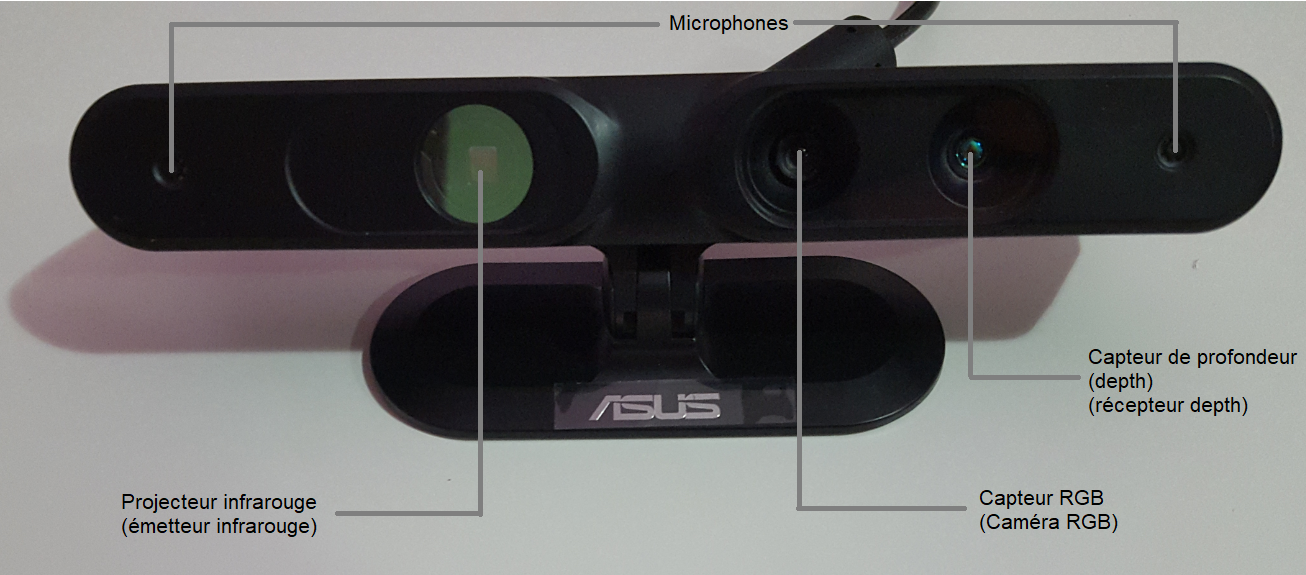
\includegraphics[scale=0.50]{images/Asus.png} \hspace{2cm}
  \caption{Composants caméra RGB-D (Ici Asus Xtion Pro Live).\label{fig-Asus}}
\end{figure}

Par la suite, les valeurs obtenues seront corrélées à un capteur RGB qu'on peut apercevoir sur la figure. Ces données pourront être représentées par un nuage de points \footnote{Est une représentation des points de coordonnées tridimensionnelles dont chacun peut avoir des attributs qui lui ont sont propres.}.


	\par Toutefois, ce type de caméras possède certaines restrictions. Parmi ces dernières, on peut citer:
	\begin{itemize}
		\item {Distances de mesure limitées.}	
		\item {Problèmes de calculs des informations de profondeur à l'encontre de surfaces brillantes, très mates, transparentes, réfléchissantes ou encore envers des objets absorbants.} 
		\item {Interférence des motifs (patterns) infrarouges si présence de plusieurs caméras RGB-D de même type. En effet, chaque capteur visualisera ses propres motifs ainsi que ceux des autres caméras présentes et ne saura distinguer les siens des autres qui se chevauchent.  De cela découle une perte considérable d'informations de profondeur comme nous pouvons l'observer sur la figure \ref{fig-interference}. 

\begin{figure}[htbp]
  %\centering
  \hspace{0.75cm}
 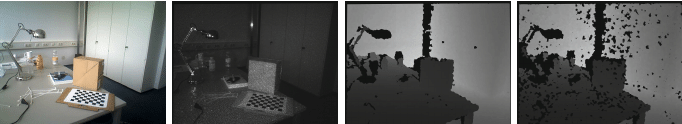
\includegraphics[scale=0.5]{images/interference.png}
  \caption{(De gauche à droite) image renvoyée par la caméra RGB, image IR, depth map (une seule caméra), depth map (deux caméras). (figure tirée de l'article de \emph{F.Alhwarin, A.Ferrein} et \emph{I.Scholl} ayant comme titre \emph{IR Stereo Kinect: Improving Depth Images by Combining StructuredLight with IR Stereo}).\label{fig-interference}}
\end{figure}

Cependant, des travaux de recherches ont été conduits afin d'y remédier. Parmi eux, on peut citer le travail réalisé par l'équipe de \emph{Rafibakhsh} ( \cite{RAFIBAKHSH15}) qui recommande de laisser un angle de 35\textdegree{} entre deux caméras suspendues à la même hauteur en considérant les scènes captées dans de bonnes conditions et une interférence très faible. \emph{Maimone} et \emph{Fuchs} \cite{MaimoneFuchs15} proposent un algorithme de remplissage et de lissage en modifiant le filtre médian aux zones trouées à l'exception des bords. Quant à \emph{F. Kenton Musgrave, Craig E.} et \emph{Robert S. Mace} \cite{KentonCraigMace12}, ils appliquent une certaine quantité minime de mouvements (en utilisant des composants matériels supplémentaires) à certains capteurs de sorte que chacun puisse voir son propre motif infrarouge de façon nette et une version floue des motifs de ses voisins. }
	\end{itemize}
\subsection{Stéréo-vision}
Une caméra stéréoscopique est un appareil qui contient deux voire plus de capteurs d'images. Ceci nous rappelle la vision binoculaire humaine. En effet, ce mécanisme permet au système nerveux central de percevoir simultanément les images issus de chaque œil envoyées sous forme de signaux. Ainsi, il sera en mesure de se servir de ces différences (entre les deux images)  pour permettre une vision stéréoscopique pour la perception de relief et une mesure des distances en utilisant la triangulation \footnote{Approche géométrique permettant une mesure des distances. Le lecteur peut consulter cette page web pour de plus amples informations: \url{https://fr.wikipedia.org/wiki/Triangulation} .}. Le concept que nous venons d'expliquer est appelé disparité stéréoscopique \footnote{Différence dans la localisation d'un objet perçu par l'œil gauche et l'œil droit résultant de la séparation horizontale des yeux dont certaines caméras essaient de s'approprier la technique afin de récupérer la profondeur.}. 
\par La stéréo-vision sert principalement à reconstituer la scène observée sous forme de modèle 3D. 
\subsubsection{Carte de disparités}
Le principe de la disparité est une approche du mécanisme humain vu précédemment. Il consiste en la différence entre les coordonnées pixels d'un point bidimensionnel d'une image et celles de son correspondant (présent sur une autre image prise au même moment). Ainsi, en appliquant le même traitement sur tous les pixels correspondants, on obtient la carte des disparités. Une carte est dite éparse lorsqu'une disparité est associée à quelques pixels et lorsque cette dernière est associée à chaque pixel, on dit d'elle qu'elle est dense.  \\ Une formule pour calculer la profondeur en fonction de la disparité s'obtient comme suit: \\ \\
\begin{equation}
 z = \dfrac{B.f}{d}  
\end{equation} 
\\ Avec: \\ \\
$z$ représentant la profondeur. \\
$B$ \emph{Baseline} représente la distance séparant les deux capteurs. \\
$f$ La distance focale en pixels calculée comme montré ci-après en nous servant de la figure \ref{fig-focal} . \\
\begin{figure}[htbp]
  %\centering
  \hspace{-3cm}
 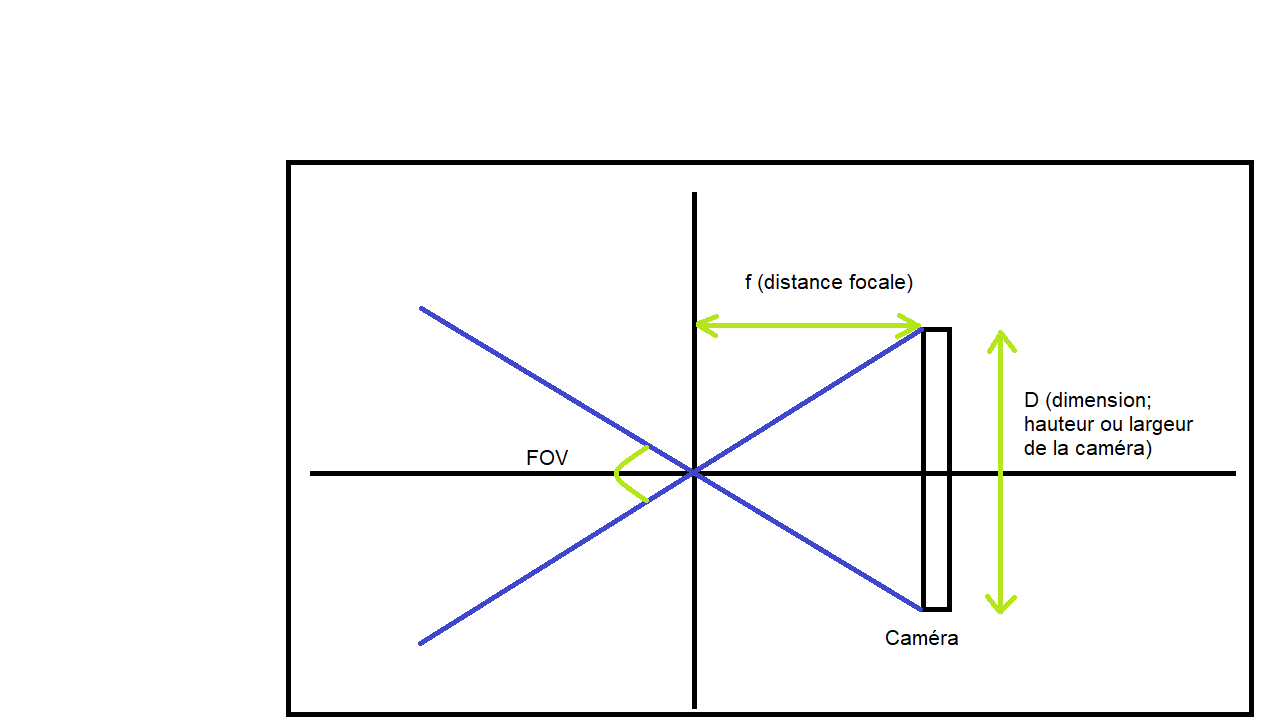
\includegraphics[scale=0.5]{images/focalLength.png} \hspace{2cm}
  \caption{Schéma illustrant la relation entre la distance focale et le champ de vision (fov).\label{fig-focal}}
\end{figure}


\begin{equation}
 \tan \left( {\dfrac{fov}{2}}\right) = \dfrac{D}{2.f}    \Leftrightarrow   f = \dfrac{D}{2. \tan \left( {\dfrac{fov}{2}}\right)}
\end{equation}
\\ Avec:\\ \\
$D$  dimension qui peut représenter soit la largeur soit la hauteur en fonction du fov de la caméra employé. \\
$fov$ (Field Of View) représente l'angle du champ de vision (soit horizontal ou vertical). \\
$f$ représente la distance focale.


\section{Kinect V2 et Kinect V3}
\subsection{Kinect V2}
\texttt{Kinect V2} se sert de la méthode TOF (ie: Time Of Flight ou autrement dit Temps De Vol) pour générer la carte de profondeur. Cette technique se base sur la différence de temps entre l'émission d'un faisceau lumineux et son retour après réflexion sur un objet. \\ La distance est calculée comme suit:\\
$ d = c.\dfrac{\Delta t}{2} $, avec $c$ la vitesse de la lumière dans l'air.\\ \par Elle permet une bien meilleure précision même dans le noir que sa version précédente (\texttt{Kinect V1)}. 

\subsection{Kinect V3}
\texttt{Kinect V3}, baptisée \texttt{Microsoft Azure Kinect V3}, tout comme la précédente version, se base aussi sur la technologie TOF. Elle comprend un capteur RGB de 12 Mp, un capteur de depth de 1Mp avec un fov réglable en large ou réduit ainsi que 7 microphones intégrés.  
 
\subsubsection{Kinect V2 Vs Kinect V3}
\texttt{Kinect V3} est beaucoup plus légère et plus petite que la \texttt{V2}. Elle possède entre autre plus de microphones que la précédente. Elle a été conçue afin d'être principalement utilisée avec Azure , le service cloud de \texttt{Microsoft}. C'est sans doute ce qui la démarque le plus de sa prédécesseure. En effet, ce service lui permet d'effectuer une partie des calculs. En outre, elle bénéficie des Cognitive Services, autrement dit de l'intelligence artificielle pourra être incluse dans les applications créées.

\chapter[Notre outil pour la qualification]{Notre outil pour la qualification de caméras RGB-D}
Dans ce passage, nous allons décrire notre outil conçu pour qualifier les caméras par rapport à notre modèle-étalon montré dans l'image ci-dessous.

\begin{figure}[htbp]
  %\centering
  \hspace{0.75cm}
 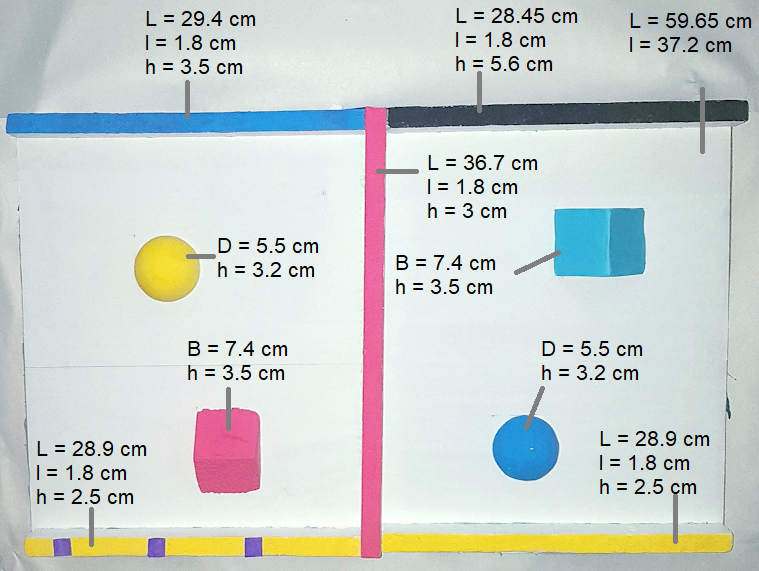
\includegraphics[scale=0.5]{images/realModel.png} \hspace{2cm}
  \caption{Modèle-étalon.\label{fig-model}}
\end{figure}

\section{Description de l'application}
Notre application est composée d'une fenêtre qui comprend une partie affichage de la scène filmée en temps réel ainsi qu'une partie interface graphique qui nous permet de communiquer avec le programme. Nous parlerons un peu plus en détail de ces parties dans les sous-sections à venir.
\subsection{Première partie: Affichage de la scène captée }
Pour cet effet, nous sommes partis d'un programme fourni par \emph{M. Farès BELHADJ} auquel nous avons rajouté des choses pour la conception de l'outil. Il comprend l'utilisation de la bibliothèque OpenGL, GL4Dummies ainsi que la bibliothèque OpenNI2 pour établir la connexion avec la caméra RGB-D pour nous fournir par la suite la carte de couleurs et la carte de profondeurs.

\subsection{Seconde partie: Interface graphique}
Pour l'interface graphique, nous avons exploité la bibliothèque Dear ImGui disponible sur GitHub sur le lien suivant \url{https://github.com/ocornut/imgui}. C'est une bibliothèque assez facile d'utilisation une fois l'étape de l'intégration dans le contexte OpenGL effectué. Cette interface contient un certain nombre de composants. Parmi les composants principaux, nous pouvons citer une liste déroulante qui nous permet de sélectionner le modèle de caméra sur laquelle nous souhaitons réaliser les tests de mesures. Ainsi, une fois le choix de caméra effectué, le programme met automatiquement à jour tous les paramètres présents dans les champs suivants la liste en récupérant les données à partir d'un fichier que nous avons nommé \emph{infoCameras.txt}. Ainsi, ce dernier pourra être exploité pour tout rajout de nouvelles caméras et/ou modification sur les données uniquement.
Autres les composants cités ci-dessus, nous noterons la présence de deux cases à cocher comme montré dans la figure \ref{fig-gui} La première permet une détection du modèle et l'autre de passer les tests de mesures.
\begin{figure}[htbp]
  %\centering
  \hspace{3.5cm}
 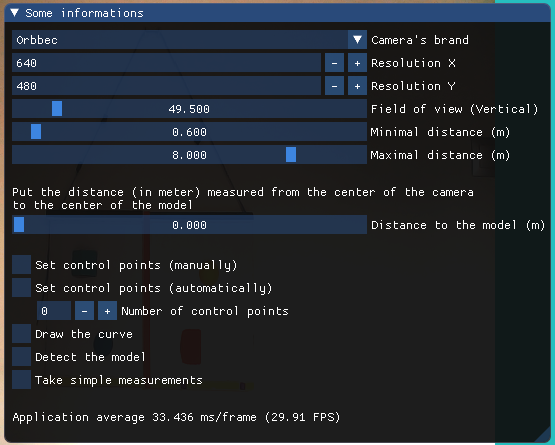
\includegraphics[scale=0.5]{images/GUI.png} \hspace{2cm}
  \caption{Interface graphique du programme.\label{fig-gui}}
\end{figure}

\subsubsection{Détection du modèle réel}  

Pour cette partie, une fonction \emph{detectObject} est prévue à cet effet afin de renvoyer la localisation du modèle réel ainsi que celles des éléments le composant (demi-sphères, "pyramides", ...), ce qui fait un total de 10 objets à identifier. Une base de données d'images est créée pour servir de templates (images modèles) afin de pouvoir les distinguer. \par Pour chacun d'entre eux, un appel à la fonction \emph{callMatchTemplate} est effectué, qui, comme son nom l'indique, appelle la fonction \emph{matchTemplate} \footnote{Fonction OpenCV permettant de trouver à partir d'une image source les zones de correspondances avec l'image \emph{template} (image modèle). La documentation sur cette fonction est disponible sur le lien suivant: \url{https://docs.opencv.org/2.4/doc/tutorials/imgproc/histograms/template_matching/template_matching.html}}. Dans cette dernière, nous transformons notre image source (image récupérée de la scène captée par la caméra RGB-D) ainsi que notre image template en niveaux de gris et ensuite nous les passons sous le filtre Canny afin de rehausser les contours pour une meilleure détection \footnote{Nous nous sommes fortement inspirés du travail réalisé par Adrian ROSEBROCK, Ph.D en vision par ordinateur, disponible sur le lien suivant: \url {https://www.pyimagesearch.com/2015/01/26/multi-scale-template-matching-using-python-opencv/}.}. Ce processus qui comprend l'utilisation des filtres est appliqué uniquement pour la détection du modèle-étalon en entier et non sur ses composants. En effet, la couleur importe pour ces derniers puisque la forme n'est pas unique (présence de deux demi-sphères, ...).
\par Cette étape est assez conséquente en terme de temps. En effet, suivant la distance à laquelle est éloignée la caméra du modèle réel, le programme doit redimensionner la scène filmée avec une certaine échelle et avec un nombre précis de fois avant d'appeler la fonction \emph{matchTemplate}, qui, combinée avec \emph{minMaxLoc}\footnote{Fonction OpenCV qui renvoie les valeurs minimales et maximales d'une \emph{Mat}. Cette dernière est une sorte de vecteur ou plus communément une matrice.}, nous permet de renvoyer la localisation du modèle-étalon (coordonnées en $x$ et $y$ ainsi que la largeur et la hauteur de l'aire détectée). 
 De ce fait, une fois les coordonnées récupérées, nous pouvons positionner notre modèle virtuel dont nous discuterons les détails de conception un peu plus loin dans ce mémoire. Ces coordonnées seront naturellement converties en coordonnées OpenGL. La formule employée à cet effet (permettant une conversion d'un système de coordonnées vers un autre) est comme suit:\\ \\
$ value_{1} = \cfrac{value - min}{max - min}.(MAX - MIN) + MIN$ \\ \\ tel que $  value\in \left[min;max\right] $ (intervalle d'entrée) et $ value_{1}\in \left[MIN;MAX\right] $ (intervalle de sortie)  \\

\begin{figure}[htbp]
  %\centering
  \hspace{5cm}
 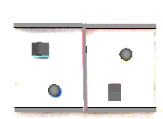
\includegraphics[scale=1]{images/modelDetected.png} \hspace{2cm}
  \caption{Positionnement du modèle 3D sur le modèle réel.\label{fig-modelDetected}}
\end{figure}

\subsubsection{Tests de mesures et rédaction de rapport}
Pour celle-ci, nous récupérons les valeurs de la carte de profondeur d'OpenGL ainsi que les valeurs de profondeur de la caméra RGB-D. les valeurs de la depth OpenGL seront par la suite linéarisées \footnote{Technique employée pour \guillemotleft{}~ approcher par une fonction linéaire ~\guillemotright{}.} et ensuite normalisées \footnote{Standardiser les données afin qu'elles appartiennent à l'intervalle $ \left[0;1\right] $.}. Celles renvoyées par la caméra seront uniquement normalisées. Les valeurs des deux côtés étant normalisées, les tests de mesures peuvent débuter. \par Pour mesurer le taux d'erreur entre les valeurs des deux profondeurs, nous avons opté pour trois méthodes distinctes; RMSE, MAPE \footnote{Mean Absolute Percentage Error est une méthode permettant une mesure des erreurs tout comme le RMSE vu plus haut. Consulter cette page web pour un maximum d'informations: \url{https://www.statisticshowto.datasciencecentral.com/mean-absolute-percentage-error-mape/} } et enfin Biais \footnote{Tout comme les deux méthodes vu précédemment, elle permet un calcul du taux d'erreur. Le lecteur peut consulter ce lien la concernant \url{http://www.chups.jussieu.fr/polys/biostats/poly/POLY.Chp.10.html}}. Une fois ces valeurs calculées pour chacun des éléments du modèle ainsi que le modèle lui-même, nous les sauvegardons dans un tableau, tableau qui sera plus tard utilisé pour le rapport. \par Par la suite, nous nous servons de Gnuplot \footnote{Un logiciel multiplateforme gratuit qui offre la possibilité de tracer des graphes en deux ou trois dimensions.} afin de tracer les graphes montrant les valeurs de depth des deux côtés en faisant attention à ne pas écraser un éventuel graphe déjà présent. 
\par De plus, un rapport est rédigé en \LaTeX{} en mettant en avant les informations relatives à la caméra ( comme le champ de vision, la résolution, ...). A chaque fois qu'on coche sur la case \textit{Do the simple measures} de l'interface graphique, le programme écrit ou réécrit sur un fichier que nous nommons \emph{Report.tex} situé dans un dossier \emph{Report} créé à cet effet. Si la caméra a déjà été testée, le programme rajoute dans la section concernée (dans le rapport) les nouveaux résultats incluant le graphe des valeurs de la profondeur, la distance calculée par le programme entre la caméra et le centre du modèle détecté ainsi qu'un tableau exposant les valeurs obtenues du taux d'erreurs pour les modèles et ses composants  avec les trois méthodes citées plus haut. Et ce, si et seulement si la caméra n'a pas été d'ores et déjà testée avec cette distance calculée par le programme.


\begin{figure}[htbp]
  %\centering
%  \hspace{5cm}
 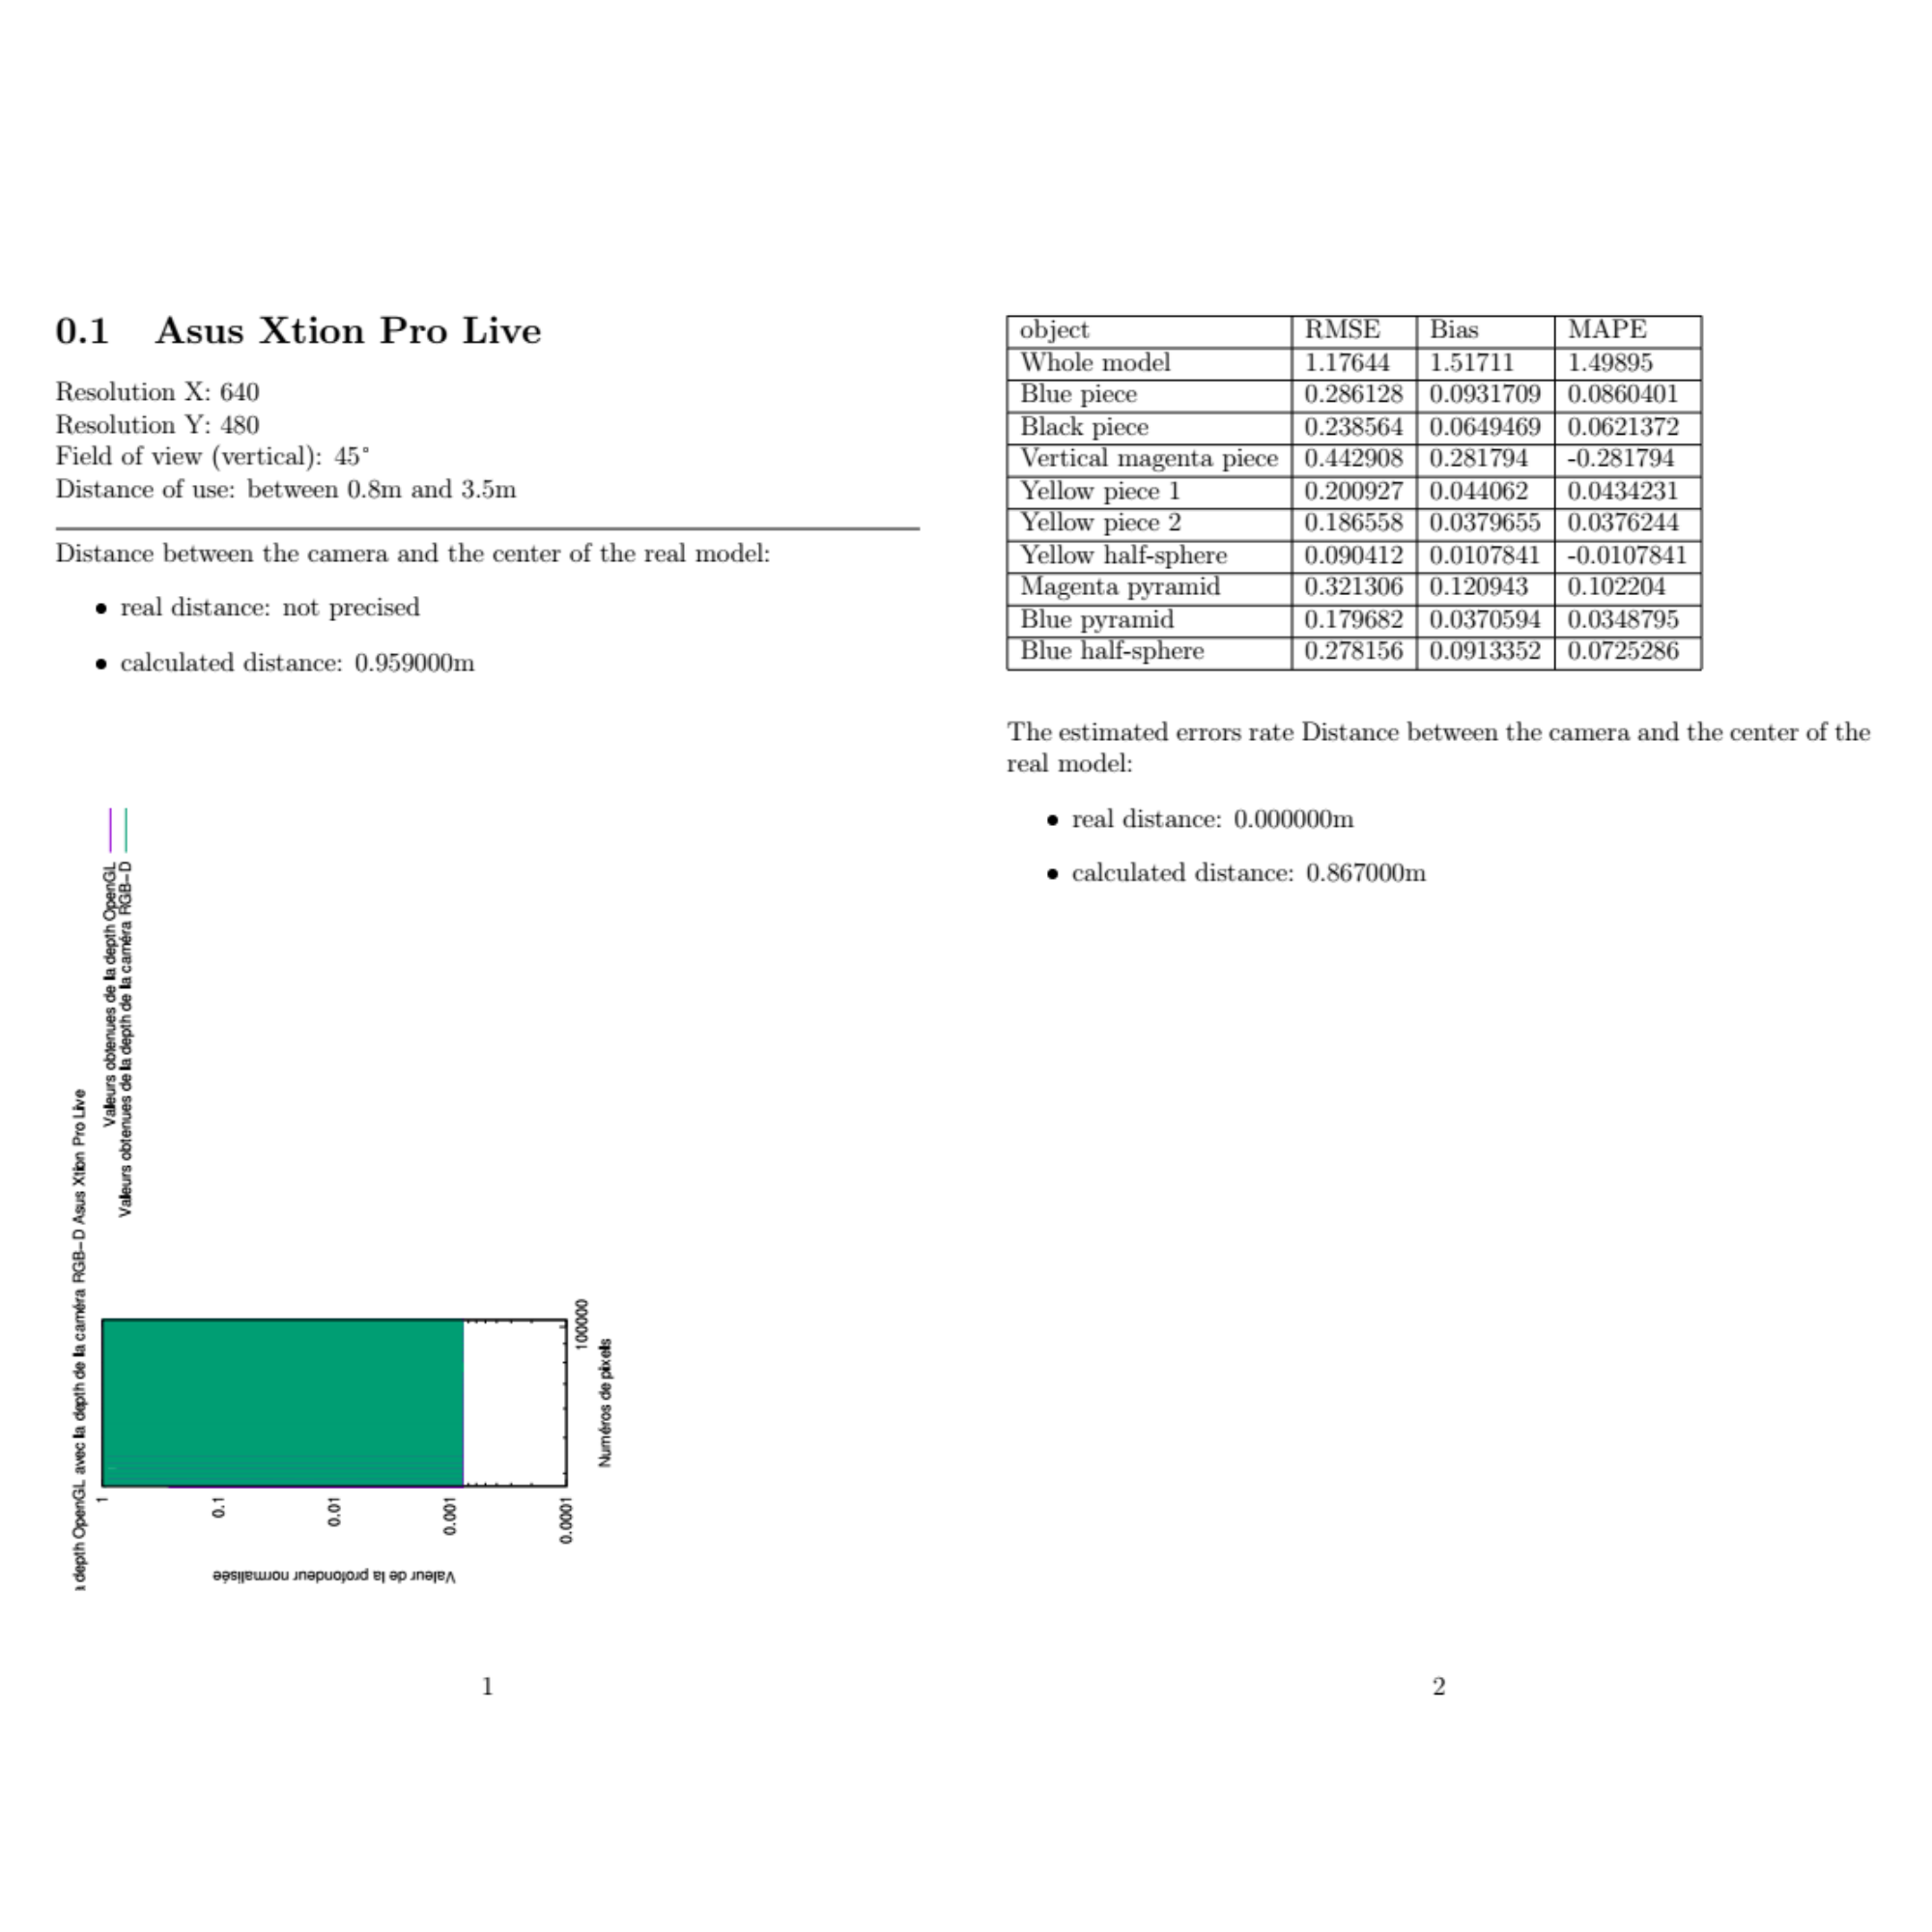
\includegraphics[scale=0.25]{images/report.png} \hspace{2cm}
  \caption{Partie du rapport généré par le programme.\label{fig-report}}
\end{figure}

\section{Conception du modèle réel et du modèle virtuel}
\subsection{Conception du modèle réel}
Pour fabriquer le modèle réel, nous avons décidé d'opter pour le polystyrène pour les composants du modèle et du carton pour sa base. Cette dernière sera par la suite recouverte de papier blanc. Les composants seront peints de couleurs distinctes suivant leur hauteur (les éléments qui possèdent une même hauteur seront peints de la même couleur plus particulièrement les rebords du modèle) sauf les demi-sphères et "pyramides".
\par Nous avons opté pour le polystyrène car c'est un matériau facilement maniable et que l'on peut trouver assez facilement.
\subsection{Conception du modèle virtuel}
La réalisation du modèle virtuel s'est faite à l'aide du logiciel 123D Design qui est assez facile d'utilisation. Chaque élément du modèle est conçu en fonction des vraies mesures faites sur le modèle réel.

\section{Comparaison de la depth OpenGL avec la depth de la caméra RGB-D}
Dans ce passage, nous exposons certains des résultats obtenus ainsi que les résultats attendus avec la caméra Asus.
\subsection{Résultats obtenus}
Ces résultats sont extraits du rapport rédigé par le programme après réalisation des tests avec la caméra Asus Xtion Pro Live avec une distance de 1.936m (distance entre la caméra et le modèle). Nous avons créé la base de données d'images templates suivant cette distance.  \\ \\

\begin{table}[H]
\begin{tabular}{c|llll}
\cline{1-4}
\multicolumn{1}{|l|}{\textbf{object}}   & \multicolumn{1}{l|}{\textbf{RMSE}} & \multicolumn{1}{l|}{\textbf{Bias}} & \multicolumn{1}{l|}{\textbf{MAPE}} &  \\
\cline{1-4}
\multicolumn{1}{|l|}{Whole model}  & \multicolumn{1}{l|}{0.645805}  & \multicolumn{1}{l|}{0.464625}  & \multicolumn{1}{l|}{0.445257}  &  \\ 
\cline{1-4}
\multicolumn{1}{|l|}{Blue piece}  & \multicolumn{1}{l|}{0.163108}  & \multicolumn{1}{l|}{0.0310855}  & \multicolumn{1}{l|}{0.0294527}  &  \\ 
\cline{1-4}
\multicolumn{1}{|l|}{Black piece}  & \multicolumn{1}{l|}{0.140734}  & \multicolumn{1}{l|}{0.0231826}  & \multicolumn{1}{l|}{0.0215494}  &  \\ 
\cline{1-4}
\multicolumn{1}{|l|}{Vertical magenta piece}  & \multicolumn{1}{l|}{0.301483}  & \multicolumn{1}{l|}{0.130255}  & \multicolumn{1}{l|}{-0.130255}  &  \\ 
\cline{1-4}
\multicolumn{1}{|l|}{Yellow piece 1}  & \multicolumn{1}{l|}{0.132736}  & \multicolumn{1}{l|}{0.019909}  & \multicolumn{1}{l|}{0.018747}  &  \\ 
\cline{1-4}
\multicolumn{1}{|l|}{Yellow piece 2}  & \multicolumn{1}{l|}{0.122078}  & \multicolumn{1}{l|}{0.0168138}  & \multicolumn{1}{l|}{0.0156804}  &  \\ 
\cline{1-4}
\multicolumn{1}{|l|}{Yellow half-sphere}  & \multicolumn{1}{l|}{0.12617}  & \multicolumn{1}{l|}{0.0215568}  & \multicolumn{1}{l|}{-0.0215568}  &  \\ 
\cline{1-4}
\multicolumn{1}{|l|}{Magenta pyramid}  & \multicolumn{1}{l|}{0.12583}  & \multicolumn{1}{l|}{0.0232983}  & \multicolumn{1}{l|}{-0.0232983}  &  \\ 
\cline{1-4}
\multicolumn{1}{|l|}{Blue pyramid}  & \multicolumn{1}{l|}{0.136497}  & \multicolumn{1}{l|}{0.0254308}  & \multicolumn{1}{l|}{-0.0254308}  &  \\ 
\cline{1-4}
\multicolumn{1}{|l|}{Blue  half-sphere}  & \multicolumn{1}{l|}{0.110225}  & \multicolumn{1}{l|}{0.0178525}  & \multicolumn{1}{l|}{-0.0178525}  &  \\ 
\cline{1-4}
\end{tabular}
\end{table}

\vspace{2cm}

Ci-dessous le tableau résumant le taux d'erreur approximatif obtenu sur des distances différentes, et ce, en  prenant en considération que la valeur RMSE  calculée. \\



\begin{table}[H]
\centering
\setlength\tabcolsep{2pt}
\begin{tabular}{c|lllllllll}
\cline{1-9}
\multicolumn{1}{|l|}{}   & 
\multicolumn{8}{l|}{\textbf{\hspace{4.5cm} Distances (m)}}    \\
\cline{1-9}
\multicolumn{1}{|l|}{\textbf{object}}   & 
\multicolumn{1}{l|}{\textbf{1.936 }} & 
\multicolumn{1}{l|}{\textbf{1.843}} & 
\multicolumn{1}{l|}{\textbf{1.748}} &  
\multicolumn{1}{l|}{\textbf{1.639 }} & 
\multicolumn{1}{l|}{\textbf{1.550}} & 
\multicolumn{1}{l|}{\textbf{1.445}} & 
\multicolumn{1}{l|}{\textbf{1.359}} & 
\multicolumn{1}{l|}{\textbf{1.259}} & \\
\cline{1-9}
\multicolumn{1}{|l|}{Whole model}  & 
\multicolumn{1}{l|}{65\%}  &  
\multicolumn{1}{l|}{69\%}  & 
\multicolumn{1}{l|}{71\%}  & 
\multicolumn{1}{l|}{76\%}  & 
\multicolumn{1}{l|}{80\%}  & 
\multicolumn{1}{l|}{84\%}  & 
\multicolumn{1}{l|}{89\%}  & 
\multicolumn{1}{l|}{94\%}  &  \\ 
\cline{1-9}
\multicolumn{1}{|l|}{Blue piece}  &
\multicolumn{1}{l|}{16\%}  &
\multicolumn{1}{l|}{17\%}  & 
\multicolumn{1}{l|}{17\%} & 
\multicolumn{1}{l|}{18\%}  & 
\multicolumn{1}{l|}{18\%}  &  
\multicolumn{1}{l|}{21\%}  & 
\multicolumn{1}{l|}{21\%}  &
\multicolumn{1}{l|}{22\%}   &  \\ 
\cline{1-9}
\multicolumn{1}{|l|}{Black piece}  & 
\multicolumn{1}{l|}{14\%}  & 
\multicolumn{1}{l|}{15\%}  & 
\multicolumn{1}{l|}{15\%} & 
\multicolumn{1}{l|}{14\%}  & 
\multicolumn{1}{l|}{17\%}  &
\multicolumn{1}{l|}{16\%}  & 
\multicolumn{1}{l|}{18\%}  & 
\multicolumn{1}{l|}{18\%}  &  \\ 
\cline{1-9}
\multicolumn{1}{|l|}{Vertical magenta piece}  & 
\multicolumn{1}{l|}{30\%}  & 
\multicolumn{1}{l|}{30\%}  & 
\multicolumn{1}{l|}{30\%} & 
\multicolumn{1}{l|}{31\%}  & 
\multicolumn{1}{l|}{31\%}  & 
\multicolumn{1}{l|}{31\%}  & 
\multicolumn{1}{l|}{32\%}  &  
\multicolumn{1}{l|}{38\%}  & \\ 
\cline{1-9}
\multicolumn{1}{|l|}{Yellow piece 1}  & 
\multicolumn{1}{l|}{13\%}  & 
\multicolumn{1}{l|}{13\%}  & 
\multicolumn{1}{l|}{13\%}  & 
\multicolumn{1}{l|}{13\%}  & 
\multicolumn{1}{l|}{13\%}  & 
\multicolumn{1}{l|}{13\%}  & 
\multicolumn{1}{l|}{13\%}  & 
\multicolumn{1}{l|}{13\%}  & \\ 
\cline{1-9}
\multicolumn{1}{|l|}{Yellow piece 2}  & 
\multicolumn{1}{l|}{12\%}  & 
\multicolumn{1}{l|}{12\%}  & 
\multicolumn{1}{l|}{12\%}  &  
\multicolumn{1}{l|}{13\%}  & 
\multicolumn{1}{l|}{13\%}  & 
\multicolumn{1}{l|}{14\%}  & 
\multicolumn{1}{l|}{12\%}  & 
\multicolumn{1}{l|}{15\%}  & \\ 
\cline{1-9}
\multicolumn{1}{|l|}{Yellow half-sphere}  & 
\multicolumn{1}{l|}{13\%}  & 
\multicolumn{1}{l|}{12\%}  & 
\multicolumn{1}{l|}{12\%}  &  
\multicolumn{1}{l|}{14\%}  & 
\multicolumn{1}{l|}{15\%}  & 
\multicolumn{1}{l|}{14\%}  & 
\multicolumn{1}{l|}{13\%}  & 
\multicolumn{1}{l|}{15\%}  & 
\\ 
\cline{1-9}
\multicolumn{1}{|l|}{Magenta pyramid}  & 
\multicolumn{1}{l|}{13\%}  & 
\multicolumn{1}{l|}{14\%}  & 
\multicolumn{1}{l|}{14\%}  &  
\multicolumn{1}{l|}{14\%}  & 
\multicolumn{1}{l|}{14\%}  & 
\multicolumn{1}{l|}{15\%}  & 
\multicolumn{1}{l|}{16\%}  & 
\multicolumn{1}{l|}{16\%}  & \\ 
\cline{1-9}
\multicolumn{1}{|l|}{Blue pyramid}  & 
\multicolumn{1}{l|}{14\%}  & 
\multicolumn{1}{l|}{14\%}  & 
\multicolumn{1}{l|}{13\%}  &  
\multicolumn{1}{l|}{13\%}  & 
\multicolumn{1}{l|}{14\%}  & 
\multicolumn{1}{l|}{16\%}  & 
\multicolumn{1}{l|}{16\%}  & 
\multicolumn{1}{l|}{17\%}  & \\ 
\cline{1-9}
\multicolumn{1}{|l|}{Blue  half-sphere}  & 
\multicolumn{1}{l|}{11\%}  & 
\multicolumn{1}{l|}{11\%}  & 
\multicolumn{1}{l|}{12\%}  &  
\multicolumn{1}{l|}{12\%}  & 
\multicolumn{1}{l|}{13\%}  & 
\multicolumn{1}{l|}{14\%}  & 
\multicolumn{1}{l|}{15\%}  & 
\multicolumn{1}{l|}{14\%}  & \\ 
\cline{1-9}
\multicolumn{1}{|l|}{\textbf{Average rate}} & 
\multicolumn{1}{l|}{\textbf{20.1\%}}  & 
\multicolumn{1}{l|}{\textbf{20.7\%}}  &  
\multicolumn{1}{l|}{\textbf{20.9\%}}  & 
\multicolumn{1}{l|}{\textbf{21.8\%}}  & 
\multicolumn{1}{l|}{\textbf{22.8\%}}  & 
\multicolumn{1}{l|}{\textbf{23.8\%}}  & 
\multicolumn{1}{l|}{\textbf{24.5\%}}  &  
\multicolumn{1}{l|}{\textbf{26.2\%}}  &\\ 
\cline{1-9}

\end{tabular}
\end{table}

\vspace{2cm} 
\par On peut observer aisément un taux d'erreur de plus en plus élevé pour le modèle en entier. Pour les autres éléments, le taux reste pratiquement constant. 

\subsection{Résultats attendus}
Comme nous doutons de la méthode employée pour extraire les données OpenGL correspondantes aux données de la depth de la caméra (données extraites aux mêmes pixels), nous pensons qu'il est tout à fait normal que le taux soit si élevé. Toutefois, comme après chaque changement de distance (ie: la caméra se rapproche du modèle observé), le modèle 3D subit un changement d'échelle afin qu'il soit superposé au modèle réel. Ainsi, la valeur de la coordonnée $z$ de chaque pixel du modèle 3D subit pareillement ce changement (devient de plus en plus grande).


\chapter{Cas pratiques de qualification}
Dans ce chapitre, nous montrons comment utiliser un modèle bien particulier de caméra avec notre application.
\section{Asus Xtion Pro Live}
Dans cette section, nous montrons comment nous avons fait pour configurer la caméra afin que le programme puisse effectuer les tests avec cette dernière.
Tout d'abord, nous avons édité le fichier \emph{infoCameras.txt} cité dans le chapitre précédent afin de pouvoir y ajouter les informations relatives à cette caméra.
\par Par la suite, nous n'avons pas eu besoin de rajouter des lignes de code pour la reconnaissance de la caméra (initialisation et récupération de la carte de couleurs et de la carte de profondeurs) car ce modèle de caméra est supporté par la bibliothèque OpenNI2.
\par Enfin, il nous suffira de sélectionner, à partir de l'interface de l'application, le modèle du capteur branché et cocher sur les cases \emph{Detect the model} pour une détection du modèle-étalon et \emph{Do the simple measures} pour démarrer les tests de mesures et rédiger le rapport comme expliqué précédemment.
\chapter{Conclusion et Perspectives\label{chap-conclusion}}
\par Dans ce rapport, nous avons présenté notre outil pour la qualification de caméras RGB-D. Comme nous avons pu le constater, cet outil recense des erreurs au niveau des mesures. En effet, des données OpenGL qui ne sont pas forcément fiables, particulièrement lors de la mise à l'échelle, influent considérablement sur les résultats que nous avons vus lors du précédent chapitre.
\par En perspectives, nous souhaiterions vérifier de manière plus pointilleuse les données OpenGL extraites et améliorer la mise à l'échelle du modèle 3D de manière à ne pas impacter le taux d'erreur.
Dans ce cas, la qualification pourra être effectuée dans des conditions permettant une meilleure comparaison entre les différents modèles de caméras.  

\nocite{*}
%	\bibliographystyle{alpha}
%\bibliography{memoire}
\printbibliography
\end{document}

